\chapter{PyPy and RPython}
PyPy consists of two parts.

The PyPy Python Interpreter ~\cite{pypy-intro} is an alternative to the standard CPython implementation that aims to closely emulate the behavior of CPython and is written in RPython. It consists of three components: (1) a bytecode compiler that takes the source code of a user application and turns it into Python code objects; (2) a Python code object interpreter; (3) a standard object space that creates or manipulates Python objects.

RPython ~\cite{rpython-doc} is a subset of Python that can be analyzed statically. The goal of the RPython toolchain is to translate RPython programs into more efficient programs for various target platforms, generally those that are considerably lower-level than Python. Compilation is carried out in the following stages:

\begin{enumerate}
\item An Annotation Pass performs a global analysis starting from a specified entry point inferring the type of each variable and building a control flow graph. Control flow graphs consist of \textit{basic blocks} that do not contain Python bytecode but rather operations after performing \textit{abstract interpretation} of the Python bytecode. Basic blocks always end with jumps to other basic blocks. After construction of the flow graph, each encountered variable is annotated with the types of all possible Python objects that can be assigned to it.

\item
The RPython Typer (or RTyper) uses the high-level information inferred during the annotation phase to turn the operations in the control flow graphs into low-level operations. At this point, function inlining, \texttt{malloc} removal and other optimizations are applied.

\item
Finally, the C backend takes the flow graphs produced by \texttt{RTyper} and produces a number of C source files that are compiled into executables.
\end{enumerate}

Throughout the thesis RPython is treated as a black box.

\section{Compile-Time Representation of RPython}

PyPltRedex works with \textbf{abstract syntax trees} and then emits RPython source code by traversing the tree and emitting strings. The abstract syntax tree is a tree that represents constructs of the language such as arithmetic operations, assignments, loops, etc.

In Python and other imperative languages, nodes of an abstract syntax tree can be split into two categories:

\begin{enumerate}
\item
Statements such as \texttt{while} and \texttt{for} loops, \texttt{if} statements, and variable assignments.
\item
Expressions such as arithmetic operations, array element access, literal values such as integers or strings, etc.
\end{enumerate}

This allows for deeply nested expressions and can be quite tedious to work with. PyPltRedex's AST definition is modified to include \texttt{PyValue} - the subset of expressions that include only variables and literals. Expressions such as additions are required to use \texttt{PyValue}, thus making resulting RPython code similar to a typical three-address code intermediate representation that most compilers employ. Figure \ref{class-diagram-rpython} shows class diagrams of all RPython abstract syntax tree nodes.

\begin{figure}[ht]
	\centering
	\makebox[\textwidth][c] { 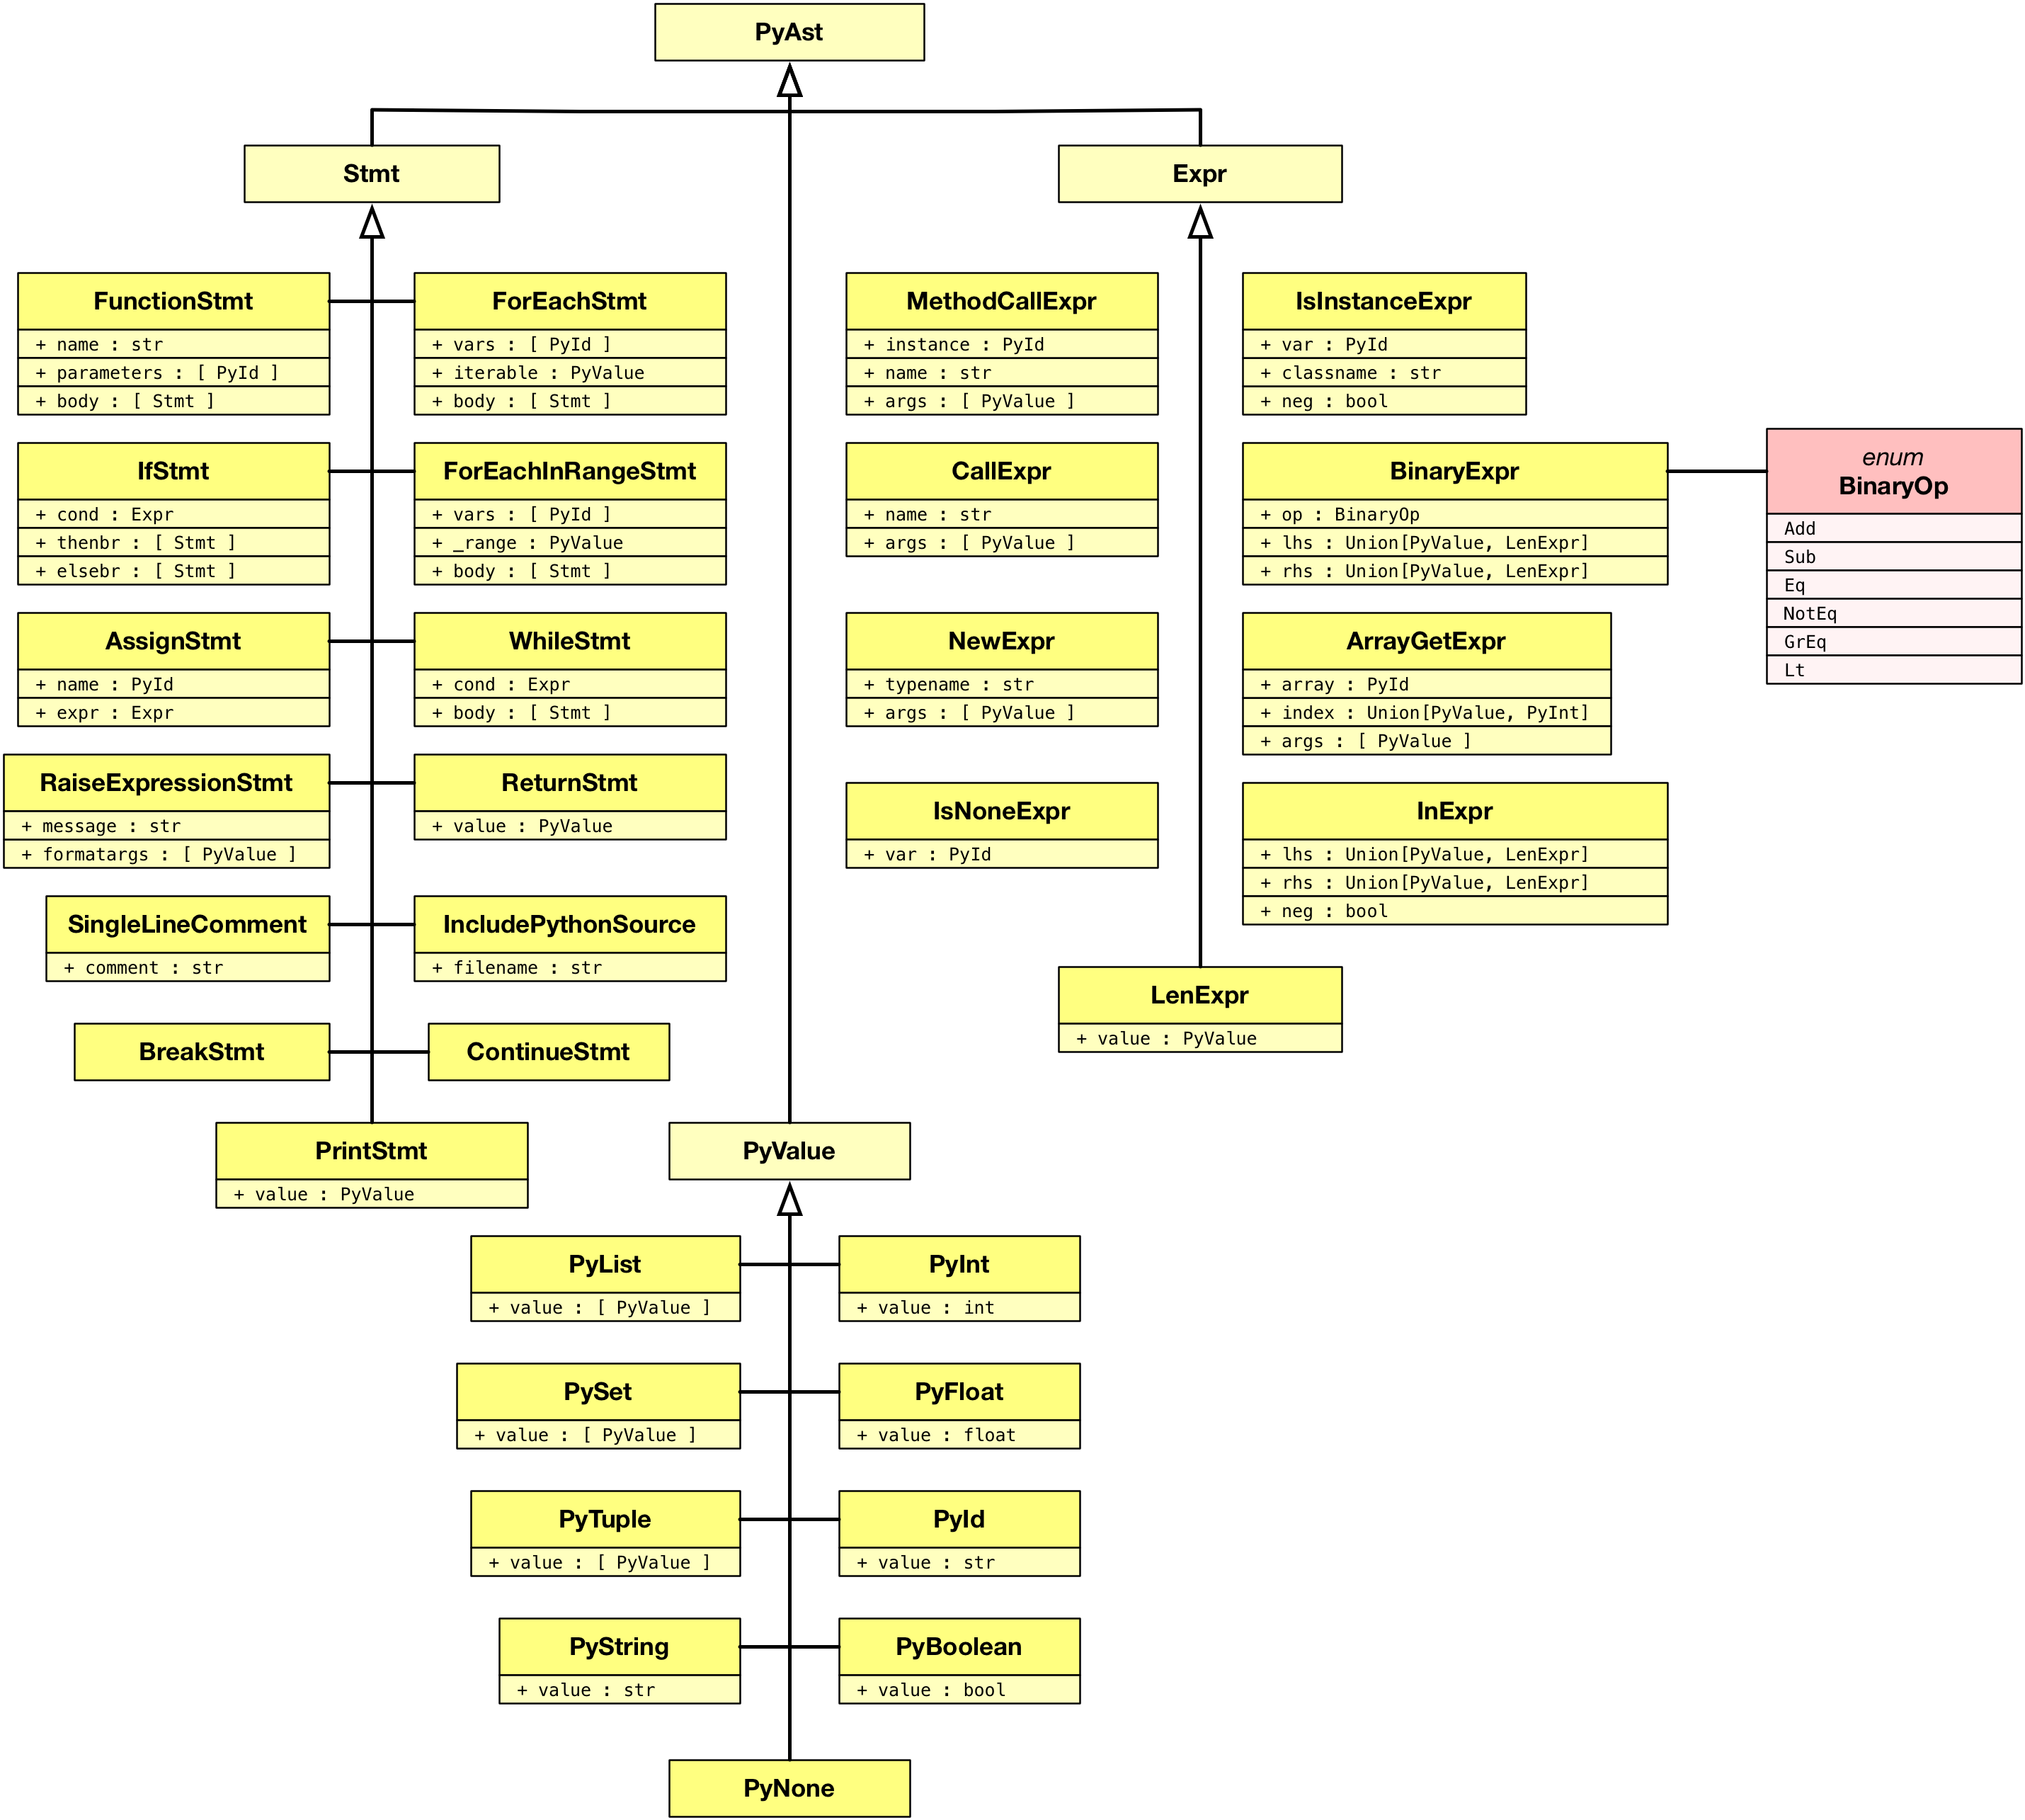
\includegraphics[scale=0.16]{class-diagram-rpython.png} }
	\caption{RPython abstract syntax tree.}
\label{class-diagram-rpython}
\end{figure}
